%% -------------------------------------------------------- %%
%%          池原研究室 2016 年度 春学期輪講用テンプレート          %%
%% -------------------------------------------------------- %%
% 
%  必要なファイル
%  (基本的にファイル移動をせず,このフォルダ内のファイルを直接
%   編集することをおすすめします)
%
%  ・serminar.tex       :  このファイル,TeX ソースの本体
%  ・ikelab-seminar.cls :  卒論 / 修論スタイルにするための各種設定
%                          このファイルを編集する必要は基本的にありません
%  ・preamble.tex       :  各種パッケージのインクルードを行います
%  ・本文中で挿入している各種画像ファイル
%    (ここでは figure ディレクトリにすべてまとめてあります)
%
\documentclass[a4paper,10pt]{ikelab-seminar}

%% スタイルの設定項目
%!TEX encoding = UTF-8 Unicode
%
% 卒論 / 修論用 プリアンブル
%

%% フォント
\usepackage{lmodern}
\usepackage[scale=0.95]{tgheros}
\usepackage{textcomp}
\usepackage[scaled=0.85]{beramono}
\usepackage[T1]{fontenc}

%% パッケージ
\usepackage[cmex10]{amsmath}
\usepackage{amssymb,amsfonts,mathtools,bm}

\usepackage{graphicx,color}
\usepackage[table]{xcolor}

\usepackage[pdfborder={0 0 0}]{hyperref}
\usepackage{pxjahyper}

% caption のコロン「図4.4: キャプション」を「図4.4 キャプション」に直す
\usepackage[labelsep=quad,compatibility=false]{caption}
\usepackage[belowskip=1.2em]{subcaption}

\usepackage{cite,url,array,makecell}
\usepackage{algorithm,algorithmic}

% 数学コマンドの補完
\DeclareMathOperator*{\sinc}{sinc}
\DeclareMathOperator*{\prox}{prox}
\DeclareMathOperator*{\argmin}{argmin}
\DeclareMathOperator*{\argmax}{argmax}

% 参考文献表示スタイルを変更
\bibliographystyle{sieicej}

% 赤色を少し暗くする
\definecolor{red}{rgb}{0.75,0,0}

\makeatletter
   % アルゴリズム図キャプションの表記を「Algorithm」→「アルゴリズム」に
   \renewcommand{\ALG@name}{アルゴリズム}
\makeatother

% 修正箇所に色付けするコマンド
%
% ・ コマンド版
%   \fixed{修正箇所}
%
% ・ 環境版
%   \begin{fixedregion}
%      修正箇所
%   \end{fixedregion}
\newcommand{\fixed}[1]{#1} 
\newenvironment{fixedregion}{\ignorespaces}{\ignorespacesafterend}
% 下の 2 行をコメントアウトすることで色付けを無効化します
\renewcommand{\fixed}[1]{\textcolor{red}{#1}}
\renewenvironment{fixedregion}{\protect\leavevmode\color{red}\ignorespaces}{\ignorespacesafterend}

% 強調
\newcommand{\strong}[1]{\textcolor{red}{\textbf{#1}}}



%% 論文タイトル
\title{\the\year 年度 春学期本輪講テンプレート}

%% 論文著者
% IEEE 系論文誌/学会誌の書式を流用しています. 他学会誌テンプレート等では
% この書式が使えないことがあるので注意して下さい

%% 1. IEEE 系ジャーナルで,著者名とメンバーシップを記述する場合
% \author{Michael~Shell,~\IEEEmembership{Member,~IEEE}}

%% 2. カンファレンス誌で,著者名およびその所属を記述する場合
\author{%
   %% IEEEauthorblockN に名前,IEEEauthorblockA に所属を書く
   \IEEEauthorblockN{Michael Shell}
   \IEEEauthorblockA{School of Electrical and \\ % \\ で改行
                     Computer Engineering \\
                     Georgia Institute of Technology, \\
                     Atlanta, Georgia 30332--0250}
   \and % (所属が 2 箇所以上あるときは \and でつなぐ)
   \IEEEauthorblockN{James Kirk and Montgomery Scott}
   \IEEEauthorblockA{Starfleet Academy \\
                     San Francisco, California 96678--2391}
}

% 出展をヘッダに書く (2 つ目の {} は使わないので空欄で)
\markboth{IEEE Transactions on Image Processing, Vol. ??, No. ??, October 20??}{}

% ------------------------------------------------------------------
\begin{document}
% タイトルを出力
\maketitle

% 概要
\begin{abstract}
この文章は池原研究室春学期最終輪講向けの \LaTeX テンプレートです.
IEEE 系論文誌のテンプレートをベースに日本語文章向けの調整を行っています.
\end{abstract}

% キーワード
\begin{IEEEkeywords}
キーワード1,キーワード2,キーワード3
\end{IEEEkeywords}

% ------------------------------------------------------------------
\section{はじめに}
\label{sec:introduction}
この文章は池原研究室春学期最終輪講向けの \LaTeX 
%            ↓ 和文の句読点には全角(,.) 英文には半角(,.) を使う
テンプレートです.
IEEE 系論文誌のテンプレートをベースに日本語文章向けの調整を行っています.
% ↓↓ 次の段落に移るには空行を入れる (次の行が字下げされる)

\ref{sec:templates}節にいくつかの文章パーツを記載しています.
参考にしてください.

\subsection{注意事項}
\begin{enumerate}
   \item フォルダ内のファイル構成を変更しないでください.\\
         (ファイルを移動するときはフォルダごと移動して下さい)
   \item ソースファイル名や画像ファイル名に日本語ファイル名,空白を含むファイル名を
         使用しないでください.
\end{enumerate}

\section{テンプレート}
\label{sec:templates}
\subsection{数式}
% $...$ の間が数式モードとなる
% 数式モード中の太字は以下の 2 コマンドで行う
%    \mathbf{(文字)} : 太字
%    \bm{(文字)}     : 太字 & 斜体
文中の数式は \verb+$...$+ で記述できる.
$x$, $\bm{y}$, $\mathbf{z}$,
% 変換で出せる記号は使わず LaTeX のコマンドで出力する
% \times は乗算記号 (×) を出力する
$256\times 256$.
一行に独立した数式は
% 下の \label{} で設定したラベルで参照できる
式 (\ref{eq:example single line}) のように記述する.
   % ← 数式の \begin の前,\end の後に空行を入れると次の段落に移動してしまう
   %   (次の文章の頭が字下げされる)
   %   段落を分けない場合は,空行を消すか,この例のように文頭に % を置く
   \begin{equation}
      \label{eq:example single line}
      y_i = \sum_{1 \leq t \leq 4} a_t x_{i \diamond t}^{(8)} + v_i
   \end{equation}
   % ←
複数行にわたる数式は \texttt{align}, \texttt{multline} を用いて書く.
   % 複数行に渡る数式は align 環境を用いて書く
   % & の位置で揃えられる
   % すべての行に番号がつくので \nonumber で抑制する
   \begin{align}
      \label{eq:example using align} 
      \hat{\bm y} = \argmin_{\bm y}
      \Biggl\{
         & \sum_{i \in W}
         \left\|
            y_i - \sum_{1 \leq t \leq 4}
            a_t x_{it}^{(8)}
         \right\|
      \Biggr. \nonumber \\ % \nonumber で数式番号を抑制,\\ で改行
      & + 
      \Biggl.
         \sum_{i \in W}
         % ノルム (2縦線) は \|...\| で記述
         \left\|
            x_i - \sum_{1 \leq t \leq 4} 
            a_t y_{it}^{(8)}
         \right\|
      \Biggr\}
   \end{align}
   % (注) \left, \right で括弧の大きさを自動的に設定できる
   %   \left(  ... \right)
   %   \left\{ ... \right\}
   %   \left[  ... \right]
   %   \left\| ... \right\|
   %
   % multline 環境は最後の行だけに番号がつく
   % align と違って & を入れない (揃える場所を指定しない) 
   \begin{multline}
     \label{eq:example using multline} 
     \hat{\bm y} = \argmin_{\bm y}
        \Biggl\{
           \sum_{i \in W}
              \left\|
                 y_i - \sum_{1 \leq t \leq 4}
                    a_t x_{it}^{(8)}
              \right\|
        \Biggr. \\ % \\ 次の行へ
     + \Biggl.
        \sum_{i \in W}
           \left\|
              x_i - \sum_{1 \leq t \leq 4}
                 a_t y_{it}^{(8)}
           \right\|
     \Biggr\}
   \end{multline}


\subsection{式や図の参照,文献の参照}
% 図表番号・式番号・節の番号への参照は \ref{ラベル} で行う
\ref{sec:introduction} 節にて $\cdots$,
(\ref{eq:example single line}) 式から $\cdots$,
図\ref{fig:example-pdf} に示す通り $\cdots$,
文献 \cite{Keys1981} によると $\cdots$,
$\cdots$ が提案されている
% 文献の引用は \cite{ラベル} で行う,複数記述できる
\cite{Keys1981,Hou1978,Jensen1995,Xin2000,Muresan2004}.

\subsection{図}
図のサンプルを図 \ref{fig:example-pdf}, \ref{fig:example-subcaption} に示します.
画像のファイル形式 PDF か PNG を用います.

%% 1 個だけの図
%   [t] 紙面の上部に配置するオプション,論文誌の場合上部に配置することが多いです
\begin{figure}[t]
   % center 環境で中央寄せする解説サイトをよく見ますが
   % 図の上下に不必要なスペースが空いてしまうので非推奨です
   % \centering を使って中央寄せしてください
   \centering
   % 画像ファイルを挿入するコマンド
   %   [width=0.8\hsize] : 幅を横幅の 0.8 倍に設定
   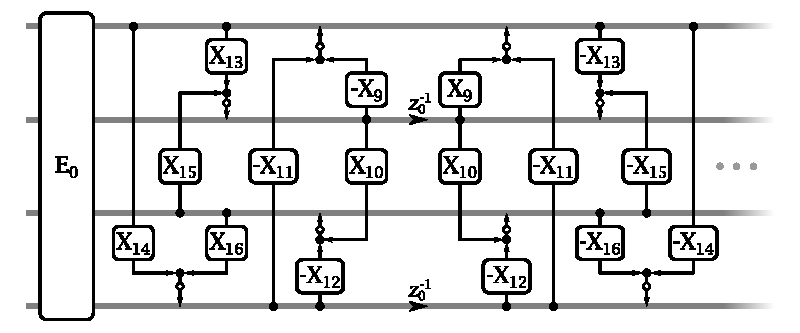
\includegraphics[width=0.8\hsize]{figure/example-pdf.pdf}
   % キャプション (図の説明)
   % 図のキャプションは,図の下に配置する
   \caption{pdf 形式の図の挿入}
   % 図番号を参照するためのラベル
   \label{fig:example-pdf}
\end{figure}

%% 複数個の図を並べて表示する例
\begin{figure}[t]
   % このように,figure の中に minipage を並べます
   % minipage の幅の合計 (0.45*2=0.9) は figure の幅より
   % 若干小さくなるようにします
   %
   %  <--------------  1  ---------------> figure の幅
   %   <---- 0.45 ---->  <---- 0.45 ---->  minipage の幅
   %     <-0.7*0.45->      <-0.7*0.45->    画像の幅
   %
   % +-------------- figure --------------+
   % | +-- minipage --+  +-- minipage --+ |
   % | | +-- image -+ |  | +-- image -+ | |
   % | | |          | |  | |          | | |
   % | | |          | |  | |          | | |
   % | | +----------+ |  | +----------+ | |
   % | | (a) Caption  |  | (b) Caption  | |
   % | +--------------+  +--------------+ |
   % |     Fig. 1  Some Caption Here      |
   % +------------------------------------+
   %
   \centering
   \begin{minipage}{.45\hsize}
      % minipage の中で再度 \centering で中央寄せする
      \centering
      % ここの .7\hsize は minipage の幅の 0.7 倍
      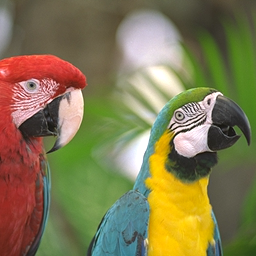
\includegraphics[width=.7\hsize]{figure/example-png.png}
      % 分けた図のキャプション  (a) ...
      \subcaption{PNG 形式の画像}
   \end{minipage}
   \begin{minipage}{.45\hsize}
      \centering
      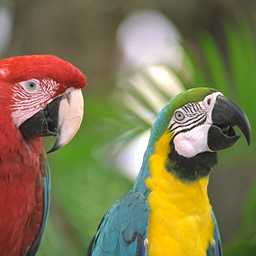
\includegraphics[width=.7\hsize]{figure/example-jpg.jpg}
      % 分けた図のキャプション  (b) ...
      \subcaption{JPEG 形式の画像}
   \end{minipage}
   % 図全体のキャプション  図 ...
   \caption{複数個の図を並べて表示}
   \label{fig:example-subcaption}
\end{figure}

%% 段組をまたぐ図は figure* で挿入できます
\begin{figure*}[t]
   \centering
   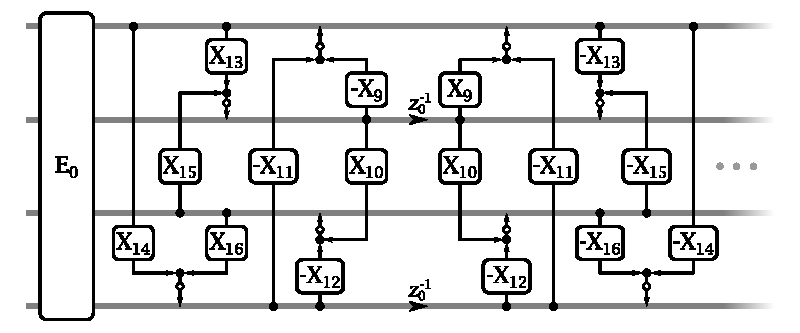
\includegraphics[width=.6\hsize]{figure/example-pdf.pdf}
   \caption{段組をまたぐ図の挿入}
\end{figure*}

\subsection{表}
表組みのサンプルを表\ref{tbl:example}および表\ref{tbl:example-span}に示します.

%% 表は table 環境で挿入します.図と同様に [t] で配置位置を丈夫に設定します
\begin{table}[t]
   \centering
   % 表のキャプションは表の上に記述する
   \caption{表のサンプル}
   \label{tbl:example}
   %               ↓ 列数と列ごとのフォーマットを指定
   %                   c:中央寄せ, |:縦方向の罫線を引く
   \begin{tabular}{c|ccc}
      % 横罫線 を引く
      \hline
      % & で次の列にうつる
      \textbf{Image}  & Bicubic  & $\cdots$ & 提案手法 \\ % \\ で次の行に
      \hline
      % \textbf{太字にする文字}, \textcolor{色}{色がつく文字}
      \textbf{Lena}   & 33.92    & $\cdots$ & \textcolor{red}{34.74} \\
      \textbf{Flower} & 32.30    & $\cdots$ & \textcolor{red}{32.51} \\
      \textbf{Leaves} & 30.52    & $\cdots$ & \textcolor{red}{32.16} \\
      $\vdots$        & $\vdots$ & $\cdots$ &    $\vdots$            \\
      \hline
      平均             & 29.87    & $\cdots$ & \textcolor{red}{30.51} \\
      \hline
   \end{tabular}
\end{table}

%% 段落をまたぐ表
\begin{table*}[t]
   \centering
   \caption{段落をまたぐ表の挿入}
   \label{tbl:example-span}
   \begin{tabular}{c|ccccc}
      \hline
      画像名   & Bicubic &  NEDI &  SAI  & 手法1 & 手法2 \\
      \hline
      Milkdrop &  30.70  & 33.70 & 33.69 & 33.99 & 33.98 \\
      \hline 
   \end{tabular}
\end{table*}


%% ----------------------------------------------------------------
%%                         参考文献リスト
%% ----------------------------------------------------------------
\begin{thebibliography}{99} % ← ここの 99 は特にいじらなくて問題ないです

   % ↓ ラベル,この論文は \cite{Muresan2000} で引用できます
   \bibitem{Muresan2000}
      % ~ は改行禁止のスペース,Fig.~1, Mr.~Tanaka 等
      D.~D.~Muresan and T.~W.~Parks, 
      % ダブルクオート開始(“)は``(バッククオート2つ)で,
      % 終了(”)は''(シングルクオート2つ)を用います
      % PDF からコピペした後は,記号を手作業で置き換える必要があります
      ``Prediction of image detail'', in 
      % \textit{斜体にする文字}
      \textit{Proc. Int. Conf. Image Processing,} vol.~2,
      % ページ範囲を表すダッシュ文字は -- で出力できます
      % PDF からコピーした - は特殊記号になっているため,置き換えが必要です
      pp.~323--326, Sep.~2000.

  \bibitem{Zhang2005} 
      X.~Wu and X.~Zhang,
      ``Image interpolation using texture orientation map 
           and kernel fisher discriminant,''
      in \textit{Proc. IEEE Int. Conf. Image Processing,} 
      Sep. 2005, vol.~1, pp.~I--49--52.

  \bibitem{Malgouyres2001} 
      F.~Malgouyres and F.~Guichard,
      ``Edge direction preserving image zooming: 
           A mathematical and numerical analysis,''
      \textit{SIAM J. Numer. Anal.,}
      vol.~39, pp.~1--37, 2001.

  \bibitem{Keys1981}
     R.~Keys,
     ``Cubic convolution interpolation for digital image processing,''
     \textit{IEEE Transactions on Acoustics, Speech and Signal Processing,}
     vol.~29, no.~6, pp.1153--1160, Dec.\ 1981.

  \bibitem{Hou1978}
     H.~S.~Hou and H.~Andrews,
     ``Cubic splines for image interpolation and digital filtering,''
     \textit{IEEE Transactions on Acoustics, Speech and Signal Processing,}
     vol.~26, no.~6, pp.508--517, Dec.\ 1978.

  \bibitem{Jensen1995}
     K.~Jensen and D.~Anastassiou,
     ``Subpixel edge localization and the interpolation of still images,''
     \textit{IEEE Transactions on Image Processing,}
     vol.~4, no.~3, pp.285--295, March 1995.

  \bibitem{Xin2000}
     X.~Li and M.~T.~Orchard,
     ``New edge directed interpolation,''
     \textit{IEEE International Conference on Image Processing,}
     vol.~2, pp.311--314, Sept.\ 2000.

  \bibitem{Muresan2004}
     D.~D. Muresan and T.~W.~Parks,
     ``Adaptively quadratic (aqua) image interpolation,''
     \textit{IEEE Transactions on Image Processing,}
     vol.~13, no.~5, pp.690--698, May 2004.

\end{thebibliography}
% ------------------------------------------------------------------

\end{document}
 
